% SDSC5001 project main report: 10 slide-style pages following Team-XX-Main-Report-Template.
% Build (run twice for page totals), from report/:
%   pdflatex -interaction=nonstopmode -aux-directory=build Team-XX-Main-Report.tex
% Figures and numbers: assets/ and assets/model_interpretation.json, written by
% project/report/make_report_assets.py from run 20261114T144053296846Z_onnx.
\documentclass[aspectratio=169,10pt,xcolor=table]{beamer}
\usepackage[T1]{fontenc}
\usepackage{lmodern}
\usepackage{booktabs,array,tikz}
\usepackage{tcolorbox}
\tcbuselibrary{skins}
\usetikzlibrary{positioning}

\definecolor{brand}{HTML}{2348D9}
\definecolor{brandsoft}{HTML}{EEF2FE}
\definecolor{ink}{HTML}{1F2633}
\definecolor{body}{HTML}{2B3340}
\definecolor{muted}{HTML}{7D8696}
\definecolor{rulegray}{HTML}{D7DCE6}
\definecolor{cardgray}{HTML}{F1F3F7}

\setbeamertemplate{navigation symbols}{}
\setbeamersize{text margin left=0.6cm,text margin right=0.6cm}
\setbeamercolor{normal text}{fg=body}
\setbeamercolor{structure}{fg=brand}
\setbeamercolor{itemize item}{fg=body}
\setbeamertemplate{itemize items}{\raisebox{1pt}{\scalebox{0.7}{\textbullet}}}
\setbeamerfont{itemize/enumerate body}{size=\footnotesize}
\setlength{\leftmargini}{1.1em}
\setbeamerfont{frametitle}{size=\large,series=\bfseries}
\setbeamertemplate{frametitle}{\vspace*{1pt}{\usebeamerfont{frametitle}\color{brand}\insertframetitle\par}\vspace{1pt}}

\newcommand{\spk}{}
\newcommand{\speakername}{HU Yuyi}
\newcommand{\ph}[1]{\textcolor{brand}{#1}}
\setbeamertemplate{headline}{\vbox{%
  \hbox{\color{brand}\rule{\paperwidth}{3pt}}%
  \hbox to \paperwidth{\hfill\rule{0pt}{8pt}{\tiny\color{muted}Speaker: \textbf{\color{brand}\speakername}
    \textperiodcentered{} \textasciitilde\spk}\hspace*{0.6cm}}}}
\setbeamertemplate{footline}{\hspace*{0.6cm}\begin{minipage}{\dimexpr\paperwidth-1.2cm\relax}
  {\color{rulegray}\rule{\linewidth}{0.4pt}}\par\vspace{1pt}
  {\tiny\color{muted}SDSC5001 Statistical Machine Learning I \textperiodcentered{} Team 100032 \textperiodcentered{}
    Learned Reranking for RAG\hfill\insertframenumber{} / \inserttotalframenumber}
  \end{minipage}\par\vspace{5pt}}

\newtcolorbox{takeaway}[1][KEY TAKEAWAY]{enhanced,colback=brandsoft,colframe=brand,boxrule=0.8pt,
  arc=2mm,left=5pt,right=5pt,top=2pt,bottom=3pt,fontupper=\footnotesize\color{ink},
  before upper={{\scriptsize\bfseries\color{brand}#1}\par\vspace{1pt}}}
\newtcolorbox{graybox}[1]{enhanced,colback=cardgray,colframe=cardgray,boxrule=0pt,
  arc=2mm,left=5pt,right=5pt,top=2pt,bottom=3pt,fontupper=\footnotesize\color{ink},
  before upper={{\scriptsize\bfseries\color{ink}#1}\par\vspace{1pt}}}
\newtcolorbox{rqcard}[1]{enhanced,colback=white,colframe=rulegray,boxrule=0.5pt,
  arc=2mm,left=5pt,right=5pt,top=3pt,bottom=4pt,fontupper=\small,
  before upper={{\bfseries\color{brand}#1}\par\vspace{1pt}}}
\newtcolorbox{figbox}{enhanced,colback=white,colframe=rulegray,boxrule=0.5pt,
  arc=1.5mm,left=2pt,right=2pt,top=2pt,bottom=2pt}
\newcommand{\fig}[1]{\begin{figbox}\centering
  \includegraphics[width=\linewidth,height=2.68cm,keepaspectratio]{#1}\end{figbox}}
\newcommand{\figcap}[1]{\par\vspace{2pt}{\scriptsize #1\par}}
\newcommand{\sect}[1]{{\small\bfseries\color{ink}#1\par}\vspace{2pt}}
\newcommand{\fnote}[1]{{\tiny\color{muted}#1\par}}
\renewcommand{\arraystretch}{1.2}

\begin{document}
% ---- 1 Title -------------------------------------------------------------
\begin{frame}[plain]
\begin{tikzpicture}[remember picture,overlay]
  \fill[brand] (current page.north west) rectangle ([xshift=5pt]current page.south west);
  \node[anchor=south east,font=\tiny,text=muted] at ([xshift=-0.6cm,yshift=0.35cm]current page.south east)
    {\insertframenumber{} / \inserttotalframenumber};
\end{tikzpicture}
\vspace*{-0.1cm}
{\scriptsize\color{muted}SDSC5001 \textperiodcentered{} Statistical Machine Learning I \textperiodcentered{} Project Report\par}
\vspace{0.25cm}
{\Large\bfseries\color{brand}Can Learned Reranking Improve Hybrid Retrieval for RAG?\par}
\vspace{0.12cm}
{\footnotesize\color{brand}TechQA Support Search: BM25 + BGE Dense Candidates, Regularized Logistic \& Random Forest Rerankers vs.\ Fixed Fusion\par}
\vspace{0.3cm}
{\scriptsize\textbf{\color{ink}Team 100032 \textperiodcentered{} Individual Presentation Parts \& Contribution Matrix:}\par}
\vspace{0.15cm}
{\scriptsize\begin{tabular}{@{}p{2.2cm}p{1.5cm}p{2.6cm}p{7.4cm}@{}}
\toprule
\textbf{Member} & \textbf{UID} & \textbf{Speaking Part} & \textbf{Key Responsibilities \& Technical Contribution}\\
\midrule
\textbf{HU Yuyi} & 60159701 & Slides 2--3  & Problem formulation, RQs, data snapshot auditing, near-duplicate quarantine\\
\textbf{Tang Yuhe} & 61034951 & Slides 4--5  & Exploratory data analysis, 256-word truncation ceiling, 3-fold grouped CV design\\
\textbf{Wang Xin} & 61023715 & Slide 6  & Pointwise L2 logistic model, feature standardization, log-odds interpretation\\
\textbf{Wang Chensu} & 60979223 & Slides 7--8 & Test benchmark, 2,000-draw bootstrap CIs, random forest importance \& PDP\\
\textbf{QUE Shenyun} & 60269510 & Slides 9--10 & 7-axis robustness checks, hard-negative sampling trap, latency \& deployment guide\\
\bottomrule
\end{tabular}\par}
\vspace{0.35cm}
{\tiny\color{muted}\textbf{Team ID:} 100032\qquad\textbf{Submission Date:} 24 November 2026\qquad\textbf{Format:} 10-Slide Action Report (5 Members, $\sim$8.0 min total)\par}
\end{frame}

% ---- 2 Motivation and RQs --------------------------------------------------
\renewcommand{\speakername}{HU Yuyi (60159701)}
\renewcommand{\spk}{0:45}
\begin{frame}{Retrieval sets the ceiling for a RAG answer; it is unclear whether a trained reranker beats fixed fusion}
\begin{columns}[T,onlytextwidth]
\begin{column}{0.49\textwidth}
\sect{Part 1: Research Motivation [HU Yuyi]}
\begin{itemize}
\item A RAG answer can only cite what retrieval returns, so evidence retrieval bounds answer quality.
\item Users: builders of a technical-support search assistant. Decision: deploy a trained reranker,
  or keep a fusion rule with two tuned constants.
\item Gap: BM25 and dense retrieval rank the same corpus differently. We do not know in advance whether a
  supervised reranker beats strong fusion on \emph{identical} candidates in this domain, or whether it
  is worth its extra latency.
\end{itemize}
\end{column}
\begin{column}{0.47\textwidth}
\begin{rqcard}{RQ1}Does the union of BM25 and dense candidates recover gold documents that either retriever misses alone?\end{rqcard}
\begin{rqcard}{RQ2}On unseen questions, does a logistic or random-forest reranker beat weighted RRF in nDCG@10 on the same candidates?\end{rqcard}
\begin{rqcard}{RQ3}Is any gain worth the extra online latency?\end{rqcard}
\end{column}
\end{columns}
\end{frame}

% ---- 3 Data ----------------------------------------------------------------
\renewcommand{\speakername}{HU Yuyi (60159701)}
\renewcommand{\spk}{0:45}
\begin{frame}{28,478 support documents and 578 questions, one judged gold each}
\begin{columns}[T,onlytextwidth]
\begin{column}{0.52\textwidth}
\sect{Part 1: Data Pipeline \& Leakage Control [HU Yuyi]}
\begin{itemize}
\item \textbf{Source:} NVIDIA TechQA-RAG-Eval archive of IBM support technotes; local snapshot audited
  12 Nov 2026 with a SHA-256 manifest, no live download.
\item \textbf{Unit:} one training row is a (question, candidate document) pair; metrics are averaged per
  question; the bootstrap resamples near-duplicate components.
\item \textbf{Response:} 1 if the candidate is the judged gold document. Unjudged candidates are proxy
  negatives, at most 50 sampled per question.
\item \textbf{Predictors (9):} BM25 and dense cosine scores; each list's reciprocal rank and missing-rank
  flag; query-term coverage; log query and document length.
\item \textbf{Known issues:} one gold per question, so Recall@20 equals hit@20; proxy negatives are not
  confirmed irrelevant; retrievers see only the first 256 words; near-duplicate grouping was
  AI-assisted, not checked by a domain expert.
\end{itemize}
\end{column}
\begin{column}{0.44\textwidth}
{\scriptsize\begin{tabular}{@{}p{4.6cm}r@{}}
\toprule
\textbf{Cleaning / split step} & \textbf{Rows left}\\
\midrule
Raw archive documents & 28,481\\
Merge exact-duplicate bodies & 28,478\\
Canonical questions & 581\\
Quarantine one cross-split component & 578\\
\rowcolor{brandsoft}\textbf{Final split: train / dev / test} & \textbf{410 / 84 / 84}\\
Independent components, dev / test & 72 / 72\\
\bottomrule
\end{tabular}\par}
\vspace{4pt}
\fnote{The historical split is locked and never re-randomised. 22,050 documents are longer than the
  256-word head (median 385 words, 95th percentile 965).}
\end{column}
\end{columns}
\end{frame}

% ---- 4 EDA -----------------------------------------------------------------
\renewcommand{\speakername}{Tang Yuhe (61034951)}
\renewcommand{\spk}{0:45}
\begin{frame}{Dense retrieval carries the signal; truncation hides tail answers}
\begin{columns}[T,onlytextwidth]
\begin{column}{0.48\textwidth}
\sect{Part 2: EDA on Retriever Signal [Tang Yuhe]}
\fig{assets/fig_dev_methods.png}
\figcap{\textbf{Shows:} on dev, dense retrieval alone (0.687) is already level with fusion and both
  rerankers (0.667--0.681). \textbf{Decision:} judge rerankers against the strongest fixed baseline,
  weighted RRF.}
\end{column}
\begin{column}{0.48\textwidth}
\sect{Part 2: 256-Word Truncation Bottleneck}
\fig{assets/fig_tail_recall.png}
\figcap{\textbf{Shows:} for 63 training questions answered after word 256, BM25 recall@100 is 0.60 on the
  head vs.\ 0.81 on full text. \textbf{Decision:} keep one shared head index; treat truncation as a
  recall ceiling for later chunking work.}
\end{column}
\end{columns}
\vspace{2pt}
\begin{takeaway}The candidate union already reaches 0.93 dev recall@100. A reranker can only reorder these
  candidates, so the room for improvement is small.\end{takeaway}
\end{frame}

% ---- 5 Model ladder and validation -----------------------------------------
\renewcommand{\speakername}{Tang Yuhe (61034951)}
\renewcommand{\spk}{0:50}
\begin{frame}{One candidate set, five methods, tuned on train and dev, tested once}
\centering
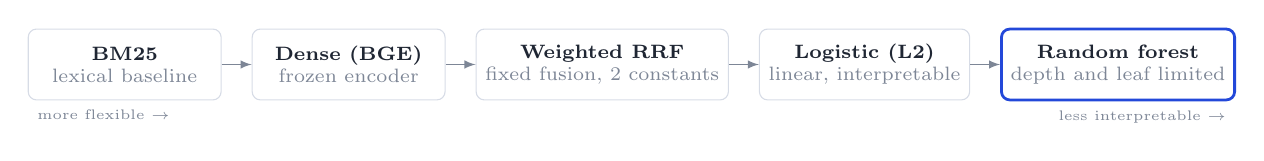
\begin{tikzpicture}[box/.style={draw=rulegray,rounded corners=3pt,minimum width=2.45cm,minimum height=0.9cm,
    align=center,font=\scriptsize,text=ink},arr/.style={-latex,draw=muted}]
\node[box] (a) {\textbf{BM25}\\{\color{muted}lexical baseline}};
\node[box,right=0.38cm of a] (b) {\textbf{Dense (BGE)}\\{\color{muted}frozen encoder}};
\node[box,right=0.38cm of b] (c) {\textbf{Weighted RRF}\\{\color{muted}fixed fusion, 2 constants}};
\node[box,right=0.38cm of c] (d) {\textbf{Logistic (L2)}\\{\color{muted}linear, interpretable}};
\node[box,right=0.38cm of d,draw=brand,line width=1pt] (e) {\textbf{Random forest}\\{\color{muted}depth and leaf limited}};
\foreach \x/\y in {a/b,b/c,c/d,d/e} \draw[arr] (\x) -- (\y);
\node[font=\tiny,text=muted,anchor=north west] at (a.south west) {more flexible $\rightarrow$};
\node[font=\tiny,text=muted,anchor=north east] at (e.south east) {less interpretable $\rightarrow$};
\end{tikzpicture}
\raggedright
\vspace{6pt}
\sect{Part 2: Grouped Validation Design [Tang Yuhe]}
\begin{itemize}
\item All methods rank the same union of BM25 and dense top-100 lists (at most 200 per question); no gold
  document is ever added to a candidate set.
\item Rerankers: 3-fold GroupKFold over near-duplicate components of the 410 training questions. Grids:
  logistic $C\in\{0.1,1,10\}$; forest depth $\{6,12\}\times$ min leaf $\{10,30\}$, 200 trees.
\item Fusion: RRF constant $k\in\{10,60,100\}$ and dense weight $\in\{0,0.25,0.5,1,2\}$, chosen on the
  84 dev questions only.
\end{itemize}
\vspace{2pt}

\begin{tikzpicture}[f/.style={draw=rulegray,rounded corners=2pt,minimum height=0.55cm,font=\scriptsize,
    text=body,inner sep=1pt}]
\foreach \i/\lab/\col in {0/fold 1/brandsoft,1/fold 2/brand!22,2/fold 3/brandsoft,3/dev: selection/brandsoft}
  \node[f,fill=\col,minimum width=2.75cm,anchor=west] at (\i*2.85,0) {\lab};
\node[f,fill=cardgray,minimum width=3.2cm,anchor=west] at (4*2.85,0) {test: used once};
\end{tikzpicture}
\par\vspace{3pt}
{\scriptsize Training set (410 questions): 3-fold grouped CV for tuning \textperiodcentered{} sampling seed
  20261114 \textperiodcentered{} metric nDCG@10, 95\% CIs from 2,000 component-paired bootstrap draws}
\end{frame}

% ---- 6 Interpretable model -------------------------------------------------
\renewcommand{\speakername}{Wang Xin (61023715)}
\renewcommand{\spk}{0:40}
\begin{frame}{The linear model relies on rank positions, not on raw retrieval scores}
\begin{columns}[T,onlytextwidth]
\begin{column}{0.55\textwidth}
\sect{Part 3: Pointwise L2 Logistic Reranker [Wang Xin]}
\begin{figbox}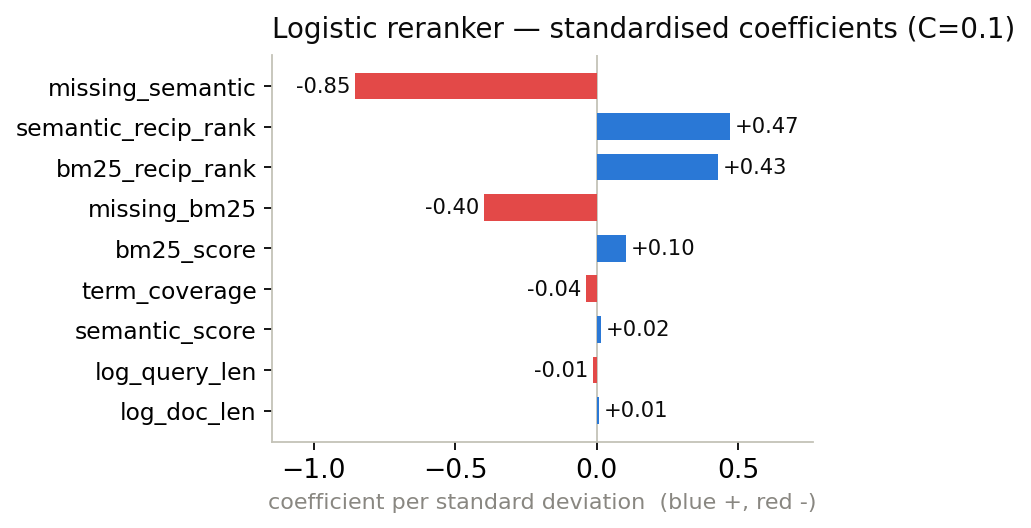
\includegraphics[width=\linewidth]{assets/fig_logistic_coef.png}\end{figbox}
\end{column}
\begin{column}{0.42\textwidth}
\begin{takeaway}The reciprocal ranks ($+0.47$ dense, $+0.43$ BM25) and the missing-rank flags ($-0.85$ dense,
  $-0.40$ BM25) carry the model. Raw scores, term coverage and lengths all lie within $\pm0.10$. The
  model mostly relearns the rank signal that RRF uses by design.\end{takeaway}
\vspace{2pt}
\begin{itemize}
\item Features standardised on training rows; L2 penalty $C=0.1$ chosen by grouped CV
  (CV nDCG@10 0.601).
\item Sign gives direction; size is the change in log-odds per standard deviation with the other
  features held fixed. Rank and score features are correlated, so read sizes loosely.
\item Scores only order candidates; with sampled negatives they are not calibrated probabilities.
\end{itemize}
\end{column}
\end{columns}
\end{frame}

% ---- 7 Model comparison ----------------------------------------------------
\renewcommand{\speakername}{Wang Chensu (60979223)}
\renewcommand{\spk}{0:55}
\begin{frame}{On the frozen test set, the logistic reranker is level with weighted RRF}
\sect{Part 4: Benchmark Comparison on Frozen Test Set [Wang Chensu]}
\begingroup\scriptsize\setlength{\tabcolsep}{4.5pt}
\begin{tabular}{@{}llrrrlrr@{}}
\toprule
\textbf{Method} & \textbf{Key hyper-parameters} & \textbf{Train CV} & \textbf{Dev} & \textbf{Test}
  & \textbf{Test $\Delta$ vs.\ W-RRF [95\% CI]} & \textbf{Test R@20} & \textbf{Median ms}\\
\midrule
BM25 & $k_1=1.2$, $b=0.75$ & -- & 0.600 & 0.510 & -- & 0.655 & 5.7\\
Dense (BGE) & bge-small-en-v1.5 & -- & 0.687 & 0.578 & -- & 0.750 & 66.5\\
RRF & $k=10$ & -- & 0.657 & 0.554 & -- & 0.726 & 71.4\\
Weighted RRF & $k=10$, dense weight 2 & -- & 0.667 & 0.585 & reference & 0.726 & 71.1\\
\rowcolor{brandsoft}\textbf{Logistic} & $C=0.1$ & 0.601 & 0.669 & 0.579
  & $\mathbf{-0.006}$ [$-0.023$, $+0.012$] & 0.738 & 69.8\\
Random forest & depth 12, leaf 10, 200 trees & 0.591 & 0.681 & 0.590
  & $+0.006$ [$-0.024$, $+0.036$] & 0.738 & 91.2\\
\bottomrule
\end{tabular}\par\endgroup
\vspace{4pt}
\fnote{nDCG@10 unless marked. Train CV: mean over 3 grouped folds. Dev: 84 questions. Test: one frozen run,
  84 questions in 72 components. Latency: median over 20 dev questions $\times$ 5 repeats per method after
  warm-up, serial, query encoding included; BGE on DirectML (RTX 3060 Laptop).}
\vspace{6pt}
\begin{takeaway}Primary comparison, fixed before test scoring: logistic minus weighted RRF in test nDCG@10 is
  $-0.006$, 95\% CI [$-0.023$, $+0.012$]. The interval includes zero, so the two methods are comparable.
  The forest's $+0.006$ is also inside noise, and its median latency is 28\% higher.\end{takeaway}
\vspace{2pt}
\fnote{The comparison and stopping rule were recorded locally before scoring, not registered externally.}
\end{frame}

% ---- 8 Drivers -------------------------------------------------------------
\renewcommand{\speakername}{Wang Chensu (60979223)}
\renewcommand{\spk}{0:55}
\begin{frame}{Both rerankers are driven by where each retriever ranked the document}
\sect{Part 4: Non-Linear Drivers \& Overfitting Analysis [Wang Chensu]}
\begin{columns}[T,onlytextwidth]
\begin{column}{0.48\textwidth}
\fig{assets/fig_rf_importance.png}
\figcap{\textbf{What matters:} the two reciprocal ranks hold 73\% of the forest's impurity importance
  (dense 0.42, BM25 0.31); term coverage (0.09) and dense score (0.08) follow.}
\end{column}
\begin{column}{0.48\textwidth}
\fig{assets/fig_rf_pdp.png}
\figcap{\textbf{How it acts:} on dev candidates, predicted relevance rises in steps as the document moves
  up either list, the same monotone pattern RRF encodes by construction.}
\end{column}
\end{columns}
\vspace{2pt}
\begin{takeaway}Of 368 training questions with the gold among the candidates, the forest leaves only 10
  outside its top 10, against 64 for logistic and 72 for weighted RRF. On the 78 such dev questions the
  counts are 13, 14 and 12: the forest's extra flexibility fits training data and does not carry over.\end{takeaway}
\end{frame}

% ---- 9 Robustness ----------------------------------------------------------
\renewcommand{\speakername}{QUE Shenyun (60269510)}
\renewcommand{\spk}{0:40}
\begin{frame}{No single analysis choice reverses the result}
\sect{Part 5: Robustness Checks \& Negative Sampling Trap [QUE Shenyun]}
\begingroup\scriptsize\setlength{\tabcolsep}{3.8pt}\renewcommand{\arraystretch}{0.98}
\begin{tabular}{@{}>{\raggedright\arraybackslash}p{2.1cm}>{\raggedright\arraybackslash}p{3.8cm}%
  >{\raggedright\arraybackslash}p{6.0cm}>{\raggedright\arraybackslash}p{1.9cm}@{}}
\toprule
\textbf{Check} & \textbf{What changed} & \textbf{Dev nDCG@10 difference [95\% CI]} & \textbf{Finding holds?}\\
\midrule
Sub-group & answer in head (66) vs.\ after or across word 256 (18); learned $-$ W-RRF
  & Logistic $+0.003$ [$-0.018$, $+0.024$] vs.\ $0.000$; RF $+0.017$ [$-0.009$, $+0.049$] vs.\ $0.000$ & Yes\\
Text policy & LSA pipelines: 256-word head $\rightarrow$ full text; logistic $-$ W-RRF
  & head $+0.003$ [$-0.003$, $+0.012$] $\rightarrow$ full $-0.004$ [$-0.010$, $+0.002$] & Yes\\
Negative cap & 50 $\rightarrow$ 10 proxy negatives per question; vs.\ main line
  & Logistic $-0.004$ [$-0.014$, $+0.001$]; RF $+0.010$ [$-0.004$, $+0.026$] & Yes\\
Class weighting & equal total weight for positives and negatives
  & Logistic $-0.007$ [$-0.021$, $+0.001$]; RF $-0.004$ [$-0.027$, $+0.019$] & Yes\\
Training seed & 20261114 $\rightarrow$ 20261115 / 20261116
  & all four $|\Delta|\le0.011$, every CI includes 0 & Yes\\
Drop features & keep only the 4 rank features
  & Logistic $+0.001$ [$0.000$, $+0.002$]; RF $-0.014$ [$-0.029$, $-0.002$] & Yes\\
Negative sampling & random $\rightarrow$ hardest unjudged BM25 hits
  & Logistic $-0.608$ [$-0.727$, $-0.478$]; RF $-0.665$ [$-0.768$, $-0.556$] & Yes, rerankers far worse\\
\bottomrule
\end{tabular}\par\endgroup
\vspace{2pt}
\begin{graybox}{WHAT MOVES THE STORY}Only hard-BM25 negatives change results sharply, for a mechanical reason:
  every hardest unjudged BM25 hit is on the BM25 list, while 32 training positives are not. Both models learn
  that \emph{absent from BM25} means relevant and fill every dev top-20 slot with such documents. The
  negative-sampling rule matters more than any hyper-parameter.\end{graybox}
\end{frame}

% ---- 10 Conclusion ---------------------------------------------------------
\renewcommand{\speakername}{QUE Shenyun (60269510)}
\renewcommand{\spk}{0:50}
\begin{frame}{Weighted RRF is enough here; the trained rerankers do not earn their cost}
\sect{Part 5: Executive Conclusion \& System Trade-offs [QUE Shenyun]}
\begin{columns}[T,onlytextwidth]
\begin{column}{0.54\textwidth}
\begin{itemize}\setlength{\itemsep}{1pt}
\item \textbf{RQ1, yes.} Dev recall@100: BM25 0.798, dense 0.905, union 0.929 (2.4 points above dense
  alone). About 7\% of dev questions still have no gold among the candidates.
\item \textbf{RQ2, no.} Test nDCG@10, logistic $-$ weighted RRF $=-0.006$ (95\% CI [$-0.023$, $+0.012$]);
  forest $+0.006$ ([$-0.024$, $+0.036$]). Neither gain is reliable.
\item \textbf{RQ3, no.} Logistic takes 69.8 ms vs.\ 71.1 ms for weighted RRF with no reliable gain; the
  forest takes 91.2 ms (+28\%).
\end{itemize}
\vspace{1pt}
\sect{Recommendations}
\begin{itemize}\setlength{\itemsep}{1pt}
\item Support-search deployment: use weighted RRF ($k=10$, dense weight 2); skip the trained reranker.
\item Raise candidate coverage first, e.g.\ by chunking long documents: no reranker can recover the
  7\% of questions whose gold is never retrieved.
\end{itemize}
\end{column}
\begin{column}{0.42\textwidth}
\begin{graybox}{LIMITATIONS}\begin{itemize}\setlength{\itemsep}{0pt}
\item One domain, one frozen encoder, first 256 words only.
\item One judged gold per question; proxy negatives are not confirmed irrelevant.
\item Grouping AI-assisted, not expert-checked; dev intervals are exploratory.
\item A local 0.5B generator gave a supported, cited answer in 1 of 5 dev cases; answer quality is not
  evaluated.
\end{itemize}\end{graybox}
\vspace{1pt}
\begin{takeaway}[FUTURE WORK]Chunk long documents and aggregate passage scores per document, developed on
  train and dev only; the test split stays frozen.\end{takeaway}
\end{column}
\end{columns}
\vspace{2pt}
\end{frame}
\end{document}

